\documentclass[border=10pt,multi,tikz]{standalone}
\usepackage{tikz}
\usetikzlibrary{mindmap}
\pagestyle{empty}
\begin{document}
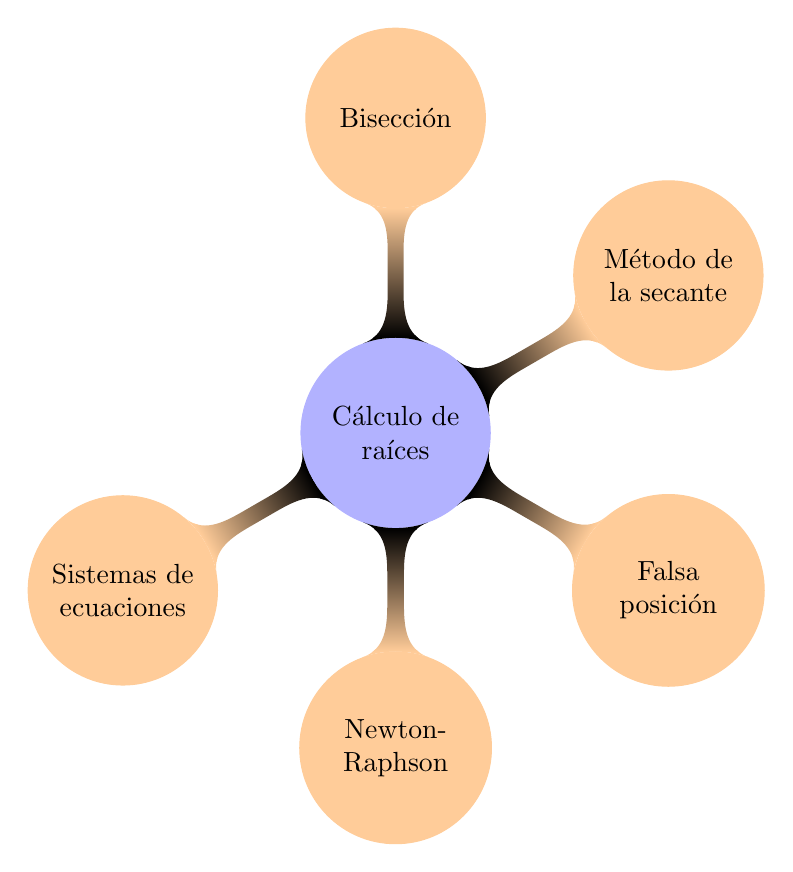
\begin{tikzpicture}[grow cyclic, text width=2cm, align=flush center, every node/.style={concept}, concept color=orange!40, 
    level 1/.style={level distance=4cm,sibling angle=60},
    level 2/.style={level distance=4cm,sibling angle=45},
    level 3/.style={level distance=4cm,sibling angle=60}]
    \node[concept color=blue!30, level distance=5cm] {Cálculo de raíces} [clockwise from=90]
        child { node {Bisección}}
        child { node {Método de la secante}}
        child { node {Falsa posición}}
        child { node {Newton-Raphson}}
        child { node {Sistemas de ecuaciones}}
;
\end{tikzpicture}
\end{document}